\documentclass[10pt,a4paper]{article}
\usepackage[utf8]{inputenc}
\usepackage[spanish, es-tabla]{babel}
\usepackage{amsmath}
\usepackage{amsfonts}
\usepackage{amssymb}
\usepackage{makeidx}
\usepackage{graphicx}
\usepackage{hyperref}
\usepackage{lmodern}
\usepackage{kpfonts}
\usepackage[left=2cm,right=2cm,top=4cm,bottom=2cm]{geometry}
\author{Daniel Vázquez Lago}
\begin{document}
\title{Tensión superficial}
\maketitle \newpage
\tableofcontents \newpage
\section{Análisis de datos}
\begin{table}[h]
\begin{center}
\begin{tabular}{|c|c|c|c|} \hline
$P  \ (N)$ & $s(P) \ (N)$ & $d \ (m)$ & $s(d) \ (m)$ 
  \\ \hline
0,069  & 0,001 & 0,063  & 0,002 
  \\  \hline
\end{tabular}
\caption{valores del peso y de el diámetro del disco con su incertidumbre}
\label{tab:masa y peso}
\end{center}
\end{table}

\subsection{Estudio de la tensión superficial a temperatura ambiente}

\begin{table}[h]
\begin{center}
\begin{tabular}{|c|c|}
\hline

medida (i) & 	 $f ' \pm 0,001 (N) $ \\ \hline
1 & 	 0,1 \\ 
2 & 	 0,099 \\ 
3 & 	 0,0995 \\ 
4 & 	 0,1 \\ 
5 & 	 0,1 \\ 
6 & 	 0,1 \\ 
7 & 	 0,0998 \\ 
8 & 	 0,1 \\ 
9 & 	 0,1 \\ 
10 & 	 0,101 \\  \hline
\end{tabular}
\caption{valores de $F'$ para el agua a temperatura ambiente (aproximadamente 22º)}
\end{center}
\label{tab:F'  }
\end{table}

\begin{table}[h!] %valores f'
\begin{center}
\begin{tabular}{|c|c|}
\hline
$F' \ (N)$ &  $s(F') \ (N)$ \\ \hline
0,09993 & 0,001 \\ \hline
\end{tabular}
\caption{Valores finales de F' y su incertidumbre}

\label{tab:valores finales F' a temperatura ambiente}
\end{center}
\end{table}

\begin{table}[h!] %tabla f
\begin{center}
\begin{tabular}{|c|c|}
\hline
$F \ (N)$ &  $s(F) \ (N)$ \\ \hline
0,0309 & 0,0014 \\ \hline
\end{tabular}
\caption{Valores finales de F y su incertidumbre}
\label{tab:valores finales F a temperatura ambiente}
\end{center}
\end{table} 

\begin{table}[h!] %tabla gamma
\begin{center}
\begin{tabular}{|c|c|}
\hline
$\gamma  \ (N/m)$ &  $s(\gamma) \ (N/m)$ \\ \hline
0,0781 & 0,0025 \\ \hline
\end{tabular}
\caption{Valores finales de $\gamma$ y su incertidumbre}

\label{tab:valores finales F a temperatura ambiente}
\end{center}
\end{table} 

\subsection{Estudio de la tensión superficial a diferentes temperaturas}
\begin{table}
\begin{center}
\begin{tabular}{|c|c|c|c|}
\hline 
medida (i) & 	 $T \pm 0,1  \ (C^o)$ & 	 $F' \pm 0,001 \ (N) $ & 	 $\gamma \pm 0,0025 \ (N/m) $ \\ \hline
1 & 	 83,1 & 	 0,088 & 	 0,0480 \\ 
2 & 	 81,1 & 	 0,089 & 	 0,0505 \\ 
3 & 	 79,3 & 	 0,0895 & 	 0,0518 \\ 
4 & 	 78,8 & 	 0,089 & 	 0,0505 \\ 
5 & 	 75,6 & 	 0,090 & 	 0,0531 \\ 
6 & 	 75,4 & 	 0,089 & 	 0,0505 \\ 
7 & 	 72,0 & 	 0,090 & 	 0,0531 \\ 
8 & 	 71,8 & 	 0,090 & 	 0,0531 \\ 
9 & 	 66,9 & 	 0,090 & 	 0,0531 \\ 
10 & 	 65,6 & 	 0,091 & 	 0,0556 \\ 
11 & 	 60,2 & 	 0,091 & 	 0,0556 \\ 
12 & 	 60,0 & 	 0,091 & 	 0,0556 \\ 
13 & 	 53,2 & 	 0,092 & 	 0,0581 \\ 
14 & 	 47,1 & 	 0,093 & 	 0,0606 \\ 
15 & 	 41,9 & 	 0,094 & 	 0,0632 \\ 
16 & 	 40,7 & 	 0,094 & 	 0,0632 \\ 
17 & 	 36,3 & 	 0,096 & 	 0,0682 \\ 
18 & 	 30,5 & 	 0,096 & 	 0,0682 \\ 
19 & 	 27,5 & 	 0,098 & 	 0,0733 \\ 
20 & 	 24,6 & 	 0,100 & 	 0,0783 \\ 
21 & 	 18,9 & 	 0,101 & 	 0,0808 \\ 
22 & 	 18,8 & 	 0,100 & 	 0,0783 \\ 
23 & 	 15,5 & 	 0,102 & 	 0,0834 \\ 
24 & 	 13,1 & 	 0,102 & 	 0,0834 \\ 
25 & 	 11,9 & 	 0,102 & 	 0,0834 \\   \hline
\end{tabular}
\caption{valores de $F'$ con diferentes temperaturas en el agua}
\label{tab:t vs f'}
\end{center}
\end{table}

\begin{figure}[h!]
\centering
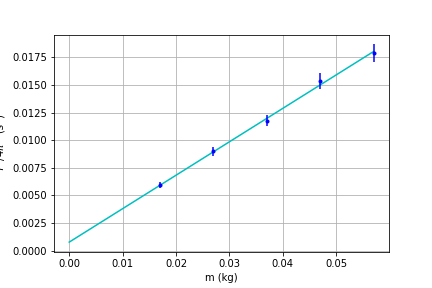
\includegraphics[width=11cm, height=7cm]{plot1.png}
\caption{Representación de $\gamma$ frente a la temperatura del agua}
\label{fig:plot1}
\end{figure}

\newpage

\subsection{Estudio de la tensión superficial con diferentes disoluciones de acetona}
\begin{table}[h] %tabla de las disoluciones
\begin{center}
\begin{tabular}{|c|c|c|c|}
\hline
medida (i) & 	 \% etanol & 	 $F' \pm 0,001  \ (N)$ & 	 $\gamma \pm 0,025 \ (N/m) $ \\ \hline
1 & 	 10 & 	 0,092 & 	 0,0581 \\ 
2 & 	 20 & 	 0,088 & 	 0,0480 \\ 
3 & 	 30 & 	 0,086 & 	 0,0429 \\ 
4 & 	 40 & 	 0,084 & 	 0,0379 \\ 
5 & 	 50 & 	 0,082 & 	 0,0328 \\ 
6 & 	 60 & 	 0,082 & 	 0,0328 \\ 
7 & 	 70 & 	 0,081 & 	 0,0303 \\ 
8 & 	 80 & 	 0,080 & 	 0,0278 \\ 
9 & 	 90 & 	 0,080 & 	 0,0278 \\ 
10 & 	 100 & 	 0,079 & 	 0,0253 \\ 

\hline

\end{tabular}
\caption{valores de $\gamma$ para diferentes disoluciones de acetona}

\label{tab:F' vs acetona}
\end{center}
\end{table}

\begin{figure}[h]
\centering
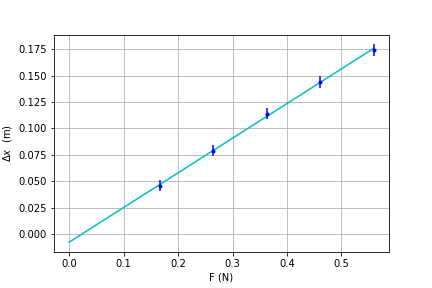
\includegraphics[width=11cm, height=7cm]{plot2.png}
\caption{Representación de $\gamma$ frente al porcentaje de acetona en la disolución}
\label{fig:plot2}
\end{figure}
\end{document}
